\documentclass[twoside,11pt]{article}

% ? Specify used packages
\usepackage{graphicx}        %  Use this one for final production.
% \usepackage[draft]{graphicx} %  Use this one for drafting.
% ? End of specify used packages

\pagestyle{myheadings}

% -----------------------------------------------------------------------------
% ? Document identification

% Fixed part
\newcommand{\stardoccategory}  {Starlink User Note}
\newcommand{\stardocinitials}  {SUN}
\newcommand{\stardocsource}    {sun\stardocnumber}

% Variable part - replace [xxx] as appropriate.
\newcommand{\stardocnumber}    {214.8}
\newcommand{\stardocauthors}   {Peter W. Draper \& Norman Gray}
\newcommand{\stardocdate}      {15 May 2000}
\newcommand{\stardoctitle}     {GAIA -- Graphical Astronomy and
                                Image Analysis Tool}
\newcommand{\stardocversion}   {2.5}
\newcommand{\stardocmanual}    {User's Manual}

\newcommand{\stardocabstract} {GAIA is an image display and analysis
tool. It provides the usual facilities of image display tools, plus
more astronomically useful ones such as aperture \& optimal
photometry, contouring, source detection, surface photometry,
arbitrary region analysis, celestial coordinate readout, calibration
and modification, grid overlays, blink comparison, defect patching and
the ability to query on-line (WWW) catalogues.}

% ? End of document identification
% -----------------------------------------------------------------------------

% +
%  Name:
%     sun.tex
%
%  Purpose:
%     Template for Starlink User Note (SUN) documents.
%     Refer to SUN/199
%
%  Authors:
%     AJC: A.J.Chipperfield (Starlink, RAL)
%     BLY: M.J.Bly (Starlink, RAL)
%     PWD: Peter W. Draper (Starlink, Durham University)
%
%  History:
%     17-JAN-1996 (AJC):
%        Original with hypertext macros, based on MDL plain originals.
%     16-JUN-1997 (BLY):
%        Adapted for LaTeX2e.
%        Added picture commands.
%     13-AUG-1998 (PWD):
%        Converted for use with LaTeX2HTML version 98.2 and
%        Star2HTML version 1.3.
%     {Add further history here}
%
% -

\newcommand{\stardocname}{\stardocinitials /\stardocnumber}
\markboth{\stardocname}{\stardocname}
\setlength{\textwidth}{160mm}
\setlength{\textheight}{230mm}
\setlength{\topmargin}{-2mm}
\setlength{\oddsidemargin}{0mm}
\setlength{\evensidemargin}{0mm}
\setlength{\parindent}{0mm}
\setlength{\parskip}{\medskipamount}
\setlength{\unitlength}{1mm}

% -----------------------------------------------------------------------------
%  Hypertext definitions.
%  ======================
%  These are used by the LaTeX2HTML translator in conjunction with star2html.

%  Comment.sty: version 2.0, 19 June 1992
%  Selectively in/exclude pieces of text.
%
%  Author
%    Victor Eijkhout                                      <eijkhout@cs.utk.edu>
%    Department of Computer Science
%    University Tennessee at Knoxville
%    104 Ayres Hall
%    Knoxville, TN 37996
%    USA

%  Do not remove the %begin{latexonly} and %end{latexonly} lines (used by
%  LaTeX2HTML to signify text it shouldn't process).
%begin{latexonly}
\makeatletter
\def\makeinnocent#1{\catcode`#1=12 }
\def\csarg#1#2{\expandafter#1\csname#2\endcsname}

\def\ThrowAwayComment#1{\begingroup
    \def\CurrentComment{#1}%
    \let\do\makeinnocent \dospecials
    \makeinnocent\^^L% and whatever other special cases
    \endlinechar`\^^M \catcode`\^^M=12 \xComment}
{\catcode`\^^M=12 \endlinechar=-1 %
 \gdef\xComment#1^^M{\def\test{#1}
      \csarg\ifx{PlainEnd\CurrentComment Test}\test
          \let\html@next\endgroup
      \else \csarg\ifx{LaLaEnd\CurrentComment Test}\test
            \edef\html@next{\endgroup\noexpand\end{\CurrentComment}}
      \else \let\html@next\xComment
      \fi \fi \html@next}
}
\makeatother

\def\includecomment
 #1{\expandafter\def\csname#1\endcsname{}%
    \expandafter\def\csname end#1\endcsname{}}
\def\excludecomment
 #1{\expandafter\def\csname#1\endcsname{\ThrowAwayComment{#1}}%
    {\escapechar=-1\relax
     \csarg\xdef{PlainEnd#1Test}{\string\\end#1}%
     \csarg\xdef{LaLaEnd#1Test}{\string\\end\string\{#1\string\}}%
    }}

%  Define environments that ignore their contents.
\excludecomment{comment}
\excludecomment{rawhtml}
\excludecomment{htmlonly}

%  Hypertext commands etc. This is a condensed version of the html.sty
%  file supplied with LaTeX2HTML by: Nikos Drakos <nikos@cbl.leeds.ac.uk> &
%  Jelle van Zeijl <jvzeijl@isou17.estec.esa.nl>. The LaTeX2HTML documentation
%  should be consulted about all commands (and the environments defined above)
%  except \xref and \xlabel which are Starlink specific.

\newcommand{\htmladdnormallinkfoot}[2]{#1\footnote{#2}}
\newcommand{\htmladdnormallink}[2]{#1}
\newcommand{\htmladdimg}[1]{}
\newcommand{\hyperref}[4]{#2\ref{#4}#3}
\newcommand{\htmlref}[2]{#1}
\newcommand{\htmlimage}[1]{}
\newcommand{\htmladdtonavigation}[1]{}

\newenvironment{latexonly}{}{}
\newcommand{\latex}[1]{#1}
\newcommand{\html}[1]{}
\newcommand{\latexhtml}[2]{#1}
\newcommand{\HTMLcode}[2][]{}

%  Starlink cross-references and labels.
\newcommand{\xref}[3]{#1}
\newcommand{\xlabel}[1]{}

%  LaTeX2HTML symbol.
\newcommand{\latextohtml}{\LaTeX2\texttt{HTML}}

%  Define command to re-centre underscore for Latex and leave as normal
%  for HTML (severe problems with \_ in tabbing environments and \_\_
%  generally otherwise).
\renewcommand{\_}{\texttt{\symbol{95}}}

% -----------------------------------------------------------------------------
%  Debugging.
%  =========
%  Remove % on the following to debug links in the HTML version using Latex.

% \newcommand{\hotlink}[2]{\fbox{\begin{tabular}[t]{@{}c@{}}#1\\\hline{\footnotesize #2}\end{tabular}}}
% \renewcommand{\htmladdnormallinkfoot}[2]{\hotlink{#1}{#2}}
% \renewcommand{\htmladdnormallink}[2]{\hotlink{#1}{#2}}
% \renewcommand{\hyperref}[4]{\hotlink{#1}{\S\ref{#4}}}
% \renewcommand{\htmlref}[2]{\hotlink{#1}{\S\ref{#2}}}
% \renewcommand{\xref}[3]{\hotlink{#1}{#2 -- #3}}
%end{latexonly}
% -----------------------------------------------------------------------------
% ? Document specific \newcommand or \newenvironment commands.
\newcommand{\mytt}[1]{{\texttt{#1}}}
\newcommand{\mybold}[1]{{\textbf{#1}}}
% ? End of document specific commands
% -----------------------------------------------------------------------------
%  Title Page.
%  ===========
\renewcommand{\thepage}{\roman{page}}
\begin{document}
\thispagestyle{empty}

%  Latex document header.
%  ======================
\begin{latexonly}
   CCLRC / \textsc{Rutherford Appleton Laboratory} \hfill \textbf{\stardocname}\\
   {\large Particle Physics \& Astronomy Research Council}\\
   {\large Starlink Project\\}
   {\large \stardoccategory\ \stardocnumber}
   \begin{flushright}
   \stardocauthors\\
   \stardocdate
   \end{flushright}
   \vspace{-4mm}
   \rule{\textwidth}{0.5mm}
   \vspace{5mm}
   \begin{center}
   {\Large\textbf{\stardoctitle \\ [2.5ex]}}
   \vspace{5mm}
% ? Add picture here if required for the LaTeX version.
   \includegraphics[totalheight=5in]{sun214fig.ps}
% ? End of picture
   \end{center}

% ? Heading for abstract if used.
   \begin{center}
      {\Large\textbf{Abstract}}
   \end{center}
% ? End of heading for abstract.
\end{latexonly}

%  HTML documentation header.
%  ==========================
\begin{htmlonly}
   \xlabel{}
   \begin{rawhtml} <H1> <FONT COLOR="#000099">\end{rawhtml}
   \begin{center}
      \stardoctitle
    \end{center}
   \begin{rawhtml} </FONT></H1> \end{rawhtml}

% ? Add picture here if required.
   \begin{center}
   \htmladdimg{sun214.jpg}
   \end{center}
% ? End of picture
   \begin{rawhtml} <P> <I> \end{rawhtml}
   \stardoccategory\ \stardocnumber \\
   \stardocauthors \\
   \stardocdate
   \begin{rawhtml} </I> </P> <H3> \end{rawhtml}
      \htmladdnormallink{CCLRC / Rutherford Appleton Laboratory}
                        {http://www.cclrc.ac.uk} \\
      \htmladdnormallink{Particle Physics \& Astronomy Research Council}
                        {http://www.pparc.ac.uk} \\
   \begin{rawhtml} </H3> <H2> \end{rawhtml}
      \htmladdnormallink{Starlink Project}{http://www.starlink.rl.ac.uk/}
   \begin{rawhtml} </H2> \end{rawhtml}
   \htmladdnormallink{\htmladdimg{source.gif} Retrieve hardcopy}
      {http://www.starlink.rl.ac.uk/cgi-bin/hcserver?\stardocsource}\\

%  HTML document table of contents.
%  ================================
%  Add table of contents header and a navigation button to return to this
%  point in the document (this should always go before the abstract \section).
  \label{stardoccontents}
  \begin{rawhtml}
    <HR>
    <H2>Contents</H2>
  \end{rawhtml}
  \htmladdtonavigation{\htmlref{\htmladdimg{contents_motif.gif}}
        {stardoccontents}}

% ? New section for abstract if used.
  \section{\xlabel{abstract}Abstract}
% ? End of new section for abstract
\end{htmlonly}

% -----------------------------------------------------------------------------
% ? Document Abstract. (if used)
%  ==================
\stardocabstract
% ? End of document abstract
% -----------------------------------------------------------------------------
% ? Latex document Table of Contents (if used).
%  ===========================================
  \newpage
  \begin{latexonly}
    \setlength{\parskip}{0mm}
    \tableofcontents
    \setlength{\parskip}{\medskipamount}
    \markboth{\stardocname}{\stardocname}
  \end{latexonly}
% ? End of Latex document table of contents
% -----------------------------------------------------------------------------
\cleardoublepage
\renewcommand{\thepage}{\arabic{page}}
\setcounter{page}{1}

% ? Main text

\section{Introduction\xlabel{introduction}\label{introduction}}

GAIA is an image display tool (c.f. SAOimage), but with the additional
capability of being extendable to integrate other programs.  At
present extensions are provided that cover the astronomically
interesting areas of aperture \& optimal photometry, automatic source
detection, surface photometry, contouring, arbitrary region analysis,
celestial coordinate readout, calibration and modification, grid
overlays, blink comparison, image defect patching and the ability to
connect to resources available in on-line (WWW) catalogues and
archives.

GAIA is a derivative of the
\htmladdnormallinkfoot{SkyCat}{http://archive.eso.org/skycat/} image
display and catalogue browsing tool, developed as part of the
\htmladdnormallinkfoot{VLT}{http://www.eso.org/vlt/} project at
\htmladdnormallinkfoot{ESO}{http://www.eso.org/}. SkyCat is free software
under the terms of the GNU copyright.

\section{\xlabel{using_gaia_from_the_cshell}Using GAIA from the C-shell}

To display an image in GAIA use the following command
(assuming that you are already initialized to use Starlink software):
\begin{quote}
\mytt{\% gaia image\_name}
\end{quote}
Alternatively you can use the \mytt{File} menu to load an image.
Information about specific toolbox windows is available in the
\mytt{Help} menus.

If you want to display an image in an existing GAIA then use the
invocation:
\begin{quote}
\mytt{\% gaiadisp image\_name}
\end{quote}
You can also write to a specific window using the clone number:
\begin{quote}
\mytt{\% gaiadisp image\_name 2}
\end{quote}
This displays into the window with title \mytt{GAIA::SkyCat (2)}. If
this window doesn't exist it will be created.

\section{\xlabel{using_gaia_from_irafcl}Using GAIA from IRAF/CL}

GAIA can be used from the IRAF/CL command-line (providing it has been
installed on your system). Before you can actually run the main program
you first need to initialize the \mytt{gaia} package:
\begin{quote}
\mytt{cl> gaia}
\end{quote}
(you could do this once and for all in your \mytt{login.cl}
file). Next you need to use the \mytt{gaiadisp} command. This command
has two arguments, the name of the image to display and the plane
({\em i.e.} GAIA clone) that you want to display into. So for instance
if you wanted to display the default IRAF test image you'd use a
command like:
\begin{quote}
\mytt{cl> gaiadisp dev\$pix.imh 1}
\end{quote}
This will either display into an existing GAIA or start up a new
instance. Note that GAIA is not an IRAF image display and will
consequently not support any IRAF cursor commands.

\section{Problems}

If you have any problems with GAIA (or suggestions for improvements),
then send an email message to
\htmladdnormallink{\mytt{gaia@star.rl.ac.uk}}{mailto:gaia@star.rl.ac.uk}.
The GAIA home page (which should have a current list of known bugs and
work arounds) is at
\htmladdnormallink{\mytt{http://www.starlink.rl.ac.uk/gaia/}}{http://www.starlink.rl.ac.uk/gaia/}.

\section{\xlabel{what_does_it_actually_do}What does it actually do?}

The capabilities of GAIA fall roughly into three areas; those of an
image display tool, those provided for the analysis of images and those
for querying on-line resources (catalogues of images and data). Each
of these areas is described very briefly in the next sections. As with
most graphical tools, probably the best way to find out about GAIA is
to explore it interactively. For specific windows (those which are
more GAIA than SkyCat) help is available on-line; many windows also
feature short one-line help descriptions of their controls.

\subsection{\xlabel{image_display_capabilities}Image Display Capabilities}
GAIA provides the following normal ``image display tool'' features:
\begin{itemize}
\item Display of images in FITS and Starlink \xref{NDF}{sun33}{}
  formats (this also means that it will display many other data formats
  using the on-the-fly data conversion ability of the NDF library, most
  notably the IRAF data format).

\item Panning, zooming, data range and colour table manipulations.

\item Continuous display of the cursor position and the image data
  value.

\item Display of many images (clones), each in its own window.

\item Coloured annotation, using text and line graphics (boxes,
  circles, polygons, lines with arrowheads, ellipses \ldots).

\item Printing of the displayed image and annotations (annotations
  are drawn using printer resolution, {\em i.e.} not a screen dump)
  to a postscript file.

\item Real time pixel value table. A table displaying the data
  values and simple statistics of a region about the cursor can be
  displayed.

\end{itemize}

\subsection{\xlabel{image_analysis_capabilities}Image Analysis Capabilities}
GAIA provides the following features, which are specifically aimed at
astronomical work with images:
\begin{itemize}
\item Aperture \& optimal photometry. A highly interactive environment
  for controlling the positions, sizes and orientations of circular
  and elliptical apertures. The sky estimates can be made from
  annuli of these apertures or from related sky apertures. The
  measurements can be in either instrumental magnitudes or
  mean counts (based on the PHOTOM - \xref{SUN/45}{sun45}{} -
  program \xref{AUTOPHOTOM}{sun45}{AUTOPHOTOM})

\item Automatic source detection. This feature provides the ability to
  automatically detect and parameterise all the objects on an
  image. These objects are then identified by displaying ellipses over
  the image and are available for interactive inspection. The resultant
  measurements are displayed in a catalogue window which can be used to
  inspect the individual values, select data on the bases of range
  limits and change the appearance of the ellipses. This is based on the
  EXTRACTOR (\xref{SUN/226}{sun226}{}) package, a derivative of
  SExtractor.

\item Extended surface photometry. This allows the interactive
  identification of extended objects (galaxies) and profile
  measurements using ellipse fitting. The resultant fits are shown
  over the images and the measurements can be inspected (based on the
  ESP - \xref{SUN/180}{sun180}{} - programs
  \xref{ELLPRO}{sun180}{ELLPRO} and \xref{ELLFOU}{sun180}{ELLFOU}).

\item Image patching. This provides the ability to select arbitrary
  shaped regions on an image and replace them with a surface fit
  to other regions, together with an artificial noise component.
  An ideal way to remove unwanted defects from an image for
  cosmetic reasons.

\item Interactive ARD (\xref{SUN/183}{sun183}{}) regions. This
  allows the calculation of statistics, the masking out and
  extraction of arbitrary shaped parts of your images as well
  defining ARD regions for other programs to use.

\item Contouring. This allows the contouring of the displayed image,
 or the overlay of contours derived from other images. The images are
 aligned using sky coordinates, if available. Control over individual
 line colours and thicknesses is provided.

\item Blink comparison. All the displayed images can be animated
  (as quickly as your hardware/CPU combination allow), or
  you can cycle through them by hand.

\item Interactive position marking: Mark and label positions on your
  images and print or record them for future reference. This also
  allows positions to be read in from text files and input sky
  coordinates to be precessed to different celestial coordinate
  systems. Mean seeing and shape parameters of any marked stars are
  also available as part of this analysis.

\item Celestial coordinates readout. If your data have suitable
  astrometric calibration data available (in recognised headers
  {\em i.e.} FITS/IRAF or NDF WCS) then a continuous readout of the
  current RA and Dec is provided.

\item Astrometric calibration. You can either fit a new
  astrometric calibration to your image (using on-line catalogues or
  images for reference positions), define a new one using known
  information (such the image scale and a reference point), copy one
  from another image and finally tweak one to make it fit better.

\item Astrometric grid overlay. If you can read out sky coordinates
  then you can also plot a grid overlay with labelled
  axes. The grid facility is provided with an enormous range of
  customization options, such as being able to change the
  celestial coordinate system (from say FK5 to  Galactic {\em etc.}).

\item Celestial coordinate system control. You can change the celestial
  coordinate system used by your image to a new one (to/from FK5,
  FK4, Ecliptic, Geocentric apparent, Galactic and SuperGalactic).

\item Sky coordinate offsets. This feature also relies on being
  able to read celestial coordinates, if so then you can
  determine the distance and offsets between any two points on
  your image (in arc minutes).

\item Real time profiling. This allows you to move a line around on
  the image and see the image data values displayed as a
  profile change. This profile can also be saved as a spectrum.

\item Object parameterization. This allows you to select a single
  object on the image. Details such as its full width half
  maximum, peak intensity {\em etc.} will be shown. These values are
  based on a 2D gaussian fit.
\end{itemize}

\subsection{\xlabel{online_catalogue_capabilities}On-line Catalogue Capabilities}
Using the facilities provided by
\htmladdnormallink{SkyCat}{http://archive.eso.org/skycat}, GAIA is
also capable of using some of the increasingly large amounts of
information available via the World Wide Web. For instance if your
image has a world coordinate system associated with it, you can query
the ESO catalogue of HST guide stars about any located within the
bounds of your image. These will then be listed and plotted over your
image.  Similarly you can query the
\htmladdnormallinkfoot{NED}{http://nedwww.ipac.caltech.edu}
(NASA/IPAC Extragalactic Database) and SAO databases (and quite a few
others) and see lists of all the objects that they know about on your
image. You can also display an image returned directly from the
\htmladdnormallinkfoot{Digital Sky Survey}
{http://arch-http.hq.eso.org/dss/dss}(and then perform queries in
other catalogues about this field). Named objects from certain
catalogues can have their full information displayed in
\htmladdnormallink{Netscape}{http://home.netscape.com} and may even
have bibliography links to the
\htmladdnormallinkfoot{ADS}{http://adswww.harvard.edu} abstract
service.  Finally the
\htmladdnormallinkfoot{HST}{http://cadcwww.dao.nrc.ca/hst} archives
are also available. Using these you can see what observations have
been made of any objects on your image (and preview any generally
available).
\begin{htmlonly}
\\
\\
\end{htmlonly}

{\bf Note:} you should take time to find what your obligations, in
terms of the correct acknowledgement of copyright, use of service
{\em etc.} are, whenever you use facilities such as those mentioned
above.

\subsection{Local catalogues}
SkyCat allows you to save its catalogue queries to a local file. These
can then be re-loaded and plotted as if on-line catalogues. This is
very useful if you need to re-plot catalogues and have a slow network,
but equally useful is the fact that local catalogues may be
modified. So you can edit, sort, select and delete records.

\subsubsection{Catalogue formats}
Local catalogues may be stored in several formats. The ``native''
version is called a ``tab separated table'' (TST). This is a simple
text file in which the values of the various fields are separated by a
single \mytt{<TAB>} character and the catalogue headers are separated
from these by a dashed line:
\begin{quote}
\begin{verbatim}
#  comment
keyword1: value1
keyword2: value2

...
ID   <TAB>   RA     <TAB>   DEC   <TAB>  MAG     ...
--           --             ---          ---
OBJ1 <TAB>   210.00 <TAB>   54.00 <TAB>  16.1
OBJ2 <TAB>   210.01 <TAB>   54.01 <TAB>  15.1
....
\end{verbatim}
\end{quote}
The usual format of a catalogue is as above, {\em i.e.} an object identifier
followed by an RA and DEC (in J2000 decimal degrees). Note the
\mytt{<TAB>} strings shouldn't be typed in, they are shown explicitly
just to make clear where they should be placed. The TST format is also
recognised by the CURSA package (\xref{SUN/190}{sun190}{}), which also
contains a description of this format.

Additional formats that can be also read by GAIA (with a performance
penalty) are those supported by the \xref{CURSA}{sun190}{} package
({\em i.e.} FITS-tables and STL format) and the ``ASCII\_HEAD'' format
of the SExtractor/EXTRACTOR package (\xref{SUN/226}{sun226}{}).

The format that is used to open or write a catalogue, is determined by
the file extension:
\begin{itemize}
\item \mybold{FITS tables}, accepted file types: \mytt{.FIT .fit .FITS .fits .GSC .gsc}
\item \mybold{STL}, accepted file types: \mytt{.TXT .txt}
\item \mybold{ASCII\_HEAD}, accepted file types: \mytt{.asc .ASC .lis .LIS}
\end{itemize}
All other file extensions are assumed to indicate a TST (the preferred
extensions for these are \mytt{.tab} or \mytt{.TAB}).

\subsubsection{Using your own local catalogues}
A useful feature of local catalogues is that you can create your own
and use GAIA to plot and manipulate them.

For instance if you wanted to plot position vectors as correctly
orientated lines over an image you would need a tab table that
contained the following sort of information:
\begin{quote}
\begin{verbatim}
# File created by: pwd on June 15, 1999 at 10:24:04
id_col: 0
x_col: 1
y_col: 2
symbol: {ID LENGTH ANGLE} {line {} {} {$ANGLE+27.0} {} {}} {{$LENGTH*0.1} {}}
#
ID      XPOS      YPOS     LENGTH    ANGLE
--      --        ---      ------    -----
ID#1    206.000   189.000  6.32528   104.816
ID#2    209.000   189.000  5.86891   109.238
\end{verbatim}
\end{quote}
The \mytt{x\_col} and \mytt{y\_col} parameters indicate the columns of
the data that correspond to the X and Y positions and the symbol
parameter how to plot a line centered on that position. In this case
the statements says extract values for the \mytt{ID}, \mytt{LENGTH}
and \mytt{ANGLE} columns, then draw lines with position angle
\mytt{ANGLE+27} and length \mytt{LENGTH$*$0.1} pixels. Note that a
dollar sign is used to prefix column names in these expressions (in
fact these expressions will be parsed by the Tcl ``expr'' command,
with the column values set to a variable with the same name as the
column for each line in the table).

Creating such a symbol parameter is best done by using the special
\mytt{Set Plot Symbols...} window, available under the local catalogue
menu \mytt{Options}. Using this window you can plot multiple symbols per
object, specify which column to use as labels, change the graphic
colour {\em etc.}. Now if you look in the file
\mytt{\~{}/.skycat/skycat.cfg} after setting up your options a suitable
symbol parameter is recorded together which the description for your
local catalogue (which you can then edit into your tab files).

To find out more about the TST format and how to configure plot
symbols you should consult the ESO document
\htmladdnormallinkfoot{``Astronomical Catalog Library''.}
{http://star-www.dur.ac.uk/\~{}pdraper/gaia/docs/cat.ps.gz}

\mybold{FITS tables:} much of the above also applies to FITS tables
that GAIA will read, {\em i.e.} FITS keywords with the names
\mytt{X\_COL}, \mytt{Y\_COL} and \mytt{SYMBOL} will be interpreted
correctly. Special parameter names that are longer than 8 characters
(such as \mytt{search\_cols}, \mytt{sort\_order}, \mytt{show\_cols}
and \mytt{copyright}) should be truncated. Long symbol expressions can
span more than one card by using the names: \mytt{SYMBOL1} through
\mytt{SYMBOL9}.

\subsection{\xlabel{image_formats}Image formats}

GAIA can display and perform analyses on many different data
formats. It does this by using the ``on-the-fly'' conversion
facilities of the NDF library, which it uses directly. This on-the-fly
conversion uses external programs that can convert your data from its
current format into an NDF and then back again (if necessary).

The CONVERT \xref{(SUN/55)}{sun55}{} package provides many formats
that are useful for astronomers (e.g. FITS, IRAF and old FIGARO
formats) and is automatically used by GAIA (unless you have set up
your own conversion facilities, see \xref{SSN/20}{ssn20}{} if you
think you need to do this). All the formats recognised at any time by
GAIA are shown in a menu in the file chooser, so check this to see
if your format is available.

FITS files are a special case in that GAIA will read these natively
(which gains increased efficiency), however, any analysis routines
(such as those used in the photometry toolbox) will still need to be
able to convert these files into NDFs, using the on-the-fly
facility, so if you define your own conversion facilities make sure
that you include a FITS converter.

\section{\xlabel{configuration_options}\label{configuration_options}Configuration options}

GAIA has many options that can be defined when starting it up. These
are set on the command line in \mytt{-option value} pairs.  Among the
more interesting are:

\hspace{2em}
\mytt{
\begin{tabular}{l|l}
 option              &  Meaning \\
\hline
 -default\_cmap      &  Change the default colour map \\
 -with\_colorramp    &  Display a colour ramp \\
 -with\_zoom\_window &  Display a zoom window \\
 -with\_pan\_window  &  Display a pan window \\
 -float\_panel       &  Detach the control panel \\
 -transient\_tools   &  Make toolboxes transient \\
 -demo\_mode         &  Make the demo toolbox available \\
 -component          &  The NDF component (data, variance or quality) \\
 -focus\_follows\_mouse & Image and entry focus follows mouse pointer \\
 -visual             & X visual to use (pseudocolor, truecolor, visual id...)
\end{tabular}
}

So for instance if you wanted to float the control panel (useful for
smaller displays) and have a grey default colourmap. Then start
using the command:
\begin{quote}
\mytt{\% gaia image\_name -default\_cmap ramp -float\_panel 1}
\end{quote}
The colour maps available can be found by listing the
\mytt{/star/bin/gaia/colormaps} directory. Or alternatively to save
some space without floating the panel try:
\begin{quote}
\mytt{\% gaia image\_name -with\_zoom\_window 0 -with\_pan\_window 0}
\end{quote}
(\mytt{1} means true and \mytt{0} false).

Alternatively you can set these in your \mytt{.Xdefaults} file:
\begin{quote}
\begin{verbatim}
*default_cmap:     ramp
*with_pan_window:  0
*with_zoom_window: 0
\end{verbatim}
\end{quote}

If you'd like the toolboxes to remain on top of the display window
they are associated with then set the \mytt{transient\_tools} option
to 1 (the precise behaviour you get depends on your window
manager). Two useful options that can only be set as X preferences
are:
\begin{quote}
\begin{verbatim}
*max_scale: 30
*min_scale: -10
\end{verbatim}
\end{quote}
These define the upper and lower limits for zooming the main
image. These are normally set to \mytt{20} and \mytt{-6}
respectively.

If you prefer to point at the image and text entry fields before using
the keyboard, rather than having to click in them first (versions of
GAIA pre-2.4 used this behaviour by default), then use the command:
\begin{quote}
\begin{verbatim}
% gaia image_name -focus_follows_mouse 1
\end{verbatim}
\end{quote}
Add this to your X preferences if you want this behaviour to be
permanent:
\begin{quote}
\begin{verbatim}
*focus_follows_mouse: 1
\end{verbatim}
\end{quote}


\subsection{\xlabel{proxy_servers}Proxy servers}
Access to the World Wide Web may be restricted (by a firewall or maybe
just site policy), so that it is only available through a ``web
cache'' or proxy server. If you are in this situation you'll need to
configure GAIA so that its remote catalogue access will work.

To do this, start up GAIA, select the \mytt{Data-Servers} menu and
choose any remote catalogue. Now in the catalogue window select the
\mytt{Options} menu and choose the \mytt{Proxies...} item.

Now fill in the two fields (consult your system administrator if you're
unclear what to enter here) and press \mytt{OK}.

\section{\xlabel{gaia_demonstration}GAIA demonstration}
Rather than just absorbing the rather dry descriptions above, you can
see some of GAIA facilities in action in a special demonstration
mode. To activate this set your current working directory to an empty
one (with several megabytes of space free). Now select the item
``Demonstration mode...'', under the ``Image-Analysis'' menu and
answer \mytt{yes} when a dialog window offering to unpack the
demonstration files appears. After a while a toolbox window will
reveal itself, just press the ``Start'' button to see the demo. Note
that the demonstration contains flashing images.

\section{\xlabel{finding_out_more_about_skycat}Finding out more about SkyCat}
\htmladdnormallink{SkyCat}{http://archive.eso.org/skycat/} is being
developed at \htmladdnormallink{ESO}{http://www.eso.org/} as part of
the \htmladdnormallink{VLT}{http://www.eso.org/vlt/} project and much
documentation is available about the internals of how SkyCat (and
consequently GAIA) are constructed. If you are interested in finding
out about these then consult the postscript documents, which you can
find from links on the \htmladdnormallinkfoot{SkyCat
homepage}{http://archive.eso.org/skycat/}. The documents relevant to
the version of SkyCat that GAIA is based on are also available at
\htmladdnormallink{http://star-www.dur.ac.uk/\~{}pdraper/gaia/docs}
{http://star-www.dur.ac.uk/~pdraper/gaia/docs}. People who would like
to extend SkyCat or GAIA at the user interface level are recommended
to read about ``SkyCat plugins''.

\section{Recent \xlabel{changes}Changes}

\subsection{Release - 2.3}
  This release includes two new toolboxes and many other enhancements.

  The new toolboxes are:
  \begin{itemize}
     \item Contouring
     \item Optimal photometry
  \end{itemize}

  The contouring toolbox allows the overlay of contours from different
  images, possibly aligned using sky coordinates (naturally it also
  allows you to contour the displayed image). It also provides control
  of the colour and line thickness of each contour.

  The optimal photometry toolbox provides facilities similar to the
  aperture photometry toolbox, both of which are based on the PHOTOM
  program AUTOPHOTOM (see \xref{SUN/45}{sun45}{}).

  The version of Skycat that GAIA is based on is now 2.4. This has
  improved catalogue facilities, an image "history" mechanism, main
  window geometry history, web proxy server dialog, histogram
  equalization, HTTP password support and many less significant changes.

  Other changes to GAIA include:
  \begin{itemize}
    \item The image panel now has quick selections for colour tables and
      intensity maps, as well as data cuts.

    \item The Sextractor toolbox is updated to work with version 2.0.19.
      This supports the new parameters:
        \begin{itemize}
           \item \mytt{BACK\_TYPE}, \mytt{BACK\_VALUE} and \mytt{THRESH\_TYPE}.
        \end{itemize}

    \item Sextractor bug fixes:
        \begin{itemize}
          \item Photometry aperture now use the given size.
          \item The messages window now only shows one copy of
                the output from Sextractor, not two.
          \item The ranges of scales in the photometry section are
                now allowed to be outside of the initial range.
        \end{itemize}

    \item A new method for transferring astrometry between images has been
      added to the \mytt{Fit to star positions...} toolbox. This works by
      selecting positions on the reference image and then selecting the
      same positions on the target image.

    \item The aperture photometry toolbox has been considerably
      reworked. Fixed apertures are now re-sizable (but keep all the
      same size) and the general layout is changed. Measurements can
      be saved and appended to a named file. You can now also change
      the aperture colours.

    \item The measure band now works when image is scrolled and zoomed.

    \item  The \mytt{pick} and \mytt{ard} toolboxes can now
           save/append their results to a file.

    \item Many others too numerous to mention.
\end{itemize}
Internally there have been many changes to GAIA, one consequence of
which is that most of the keyboard shortcuts are changed. Most
notably the interactive slice is now bound to \mytt{<control-a>}.

\subsection{Release - 2.4}
This is a minor release of GAIA that includes a new toolbox and some
minor improvements/fixes.

The new toolbox provides an interactive environment for doing the
surface photometry of extended sources ({\em i.e.} galaxies) and inspecting
the results. It is based on the ESP (\xref{SUN/180}{sun180}{}) package
commands ELLPRO and ELLFOU.

This is a minor update to GAIA with the following fixes:
\begin{itemize}
\item It is expected that work to make the
      \htmladdnormallinkfoot{LEDAS}{http://ledas-www.star.le.ac.uk/}
      catalogues available should be completed by the time of this
      release (these will appear in the ``Browse Catalog
      Directories...'' item under the ``Data-Servers'' menu).

\item A new configuration option \mytt{-focus\_follows\_mouse} has been
      added. This follows complaints from users of Solaris CDE that
      the window manager default configuration allows pop-up windows
      to disappear (behind the main window) and sometime flash
      uncontrollably. To stop this happening by default means that
      everyone will now need to point at a text entry field and click
      in it before changing the text and also click in the main window
      before scrolling using the arrow keys. To restore the old
      behaviour see
      \hyperref{configuration options}{\S}{}{configuration_options}.

\item A percentiles option has been added to automatic contour
      generation.

\item The ``automatic'' generation option now correctly uses the image
      to be contoured not the displayed image.

\item The measure band can now display pixels and non-celestial
      coordinate system offsets.

\item The SExtractor toolbox increment and decrement arrows now work
      the ``obvious'' way around.

\item Automatic NDF history recording should be working again.

\item NDFs stored within container files are now supported.

\item Floating point images of size $35,000*2,048$ pixels are now known to
      display (if you have sufficient VM). Bigger images may also work.

\item Pixel coordinates (which include the NDF origin) can now be
      selected as the ``celestial'' coordinate system (see the
      ``Celestial coordinates...'' toolbox)

\item Blank pixels in unsigned word NDFs should be be handled
      correctly.

\item It should now be possible to plot POLPACK polarization data
      again, although X and Y coordinates should still not include any
      NDF origin offsets.

\item The on-line help for the photometry toolbox is available
      again.

\item The ability to zoom around an object in the main display has
      been added (this is controlled using Shift-1 and Shift-2 mouse
      buttons).

\end{itemize}

\subsection{This release - 2.5}
  This release includes a new toolbox and some improvements and bug
  fixes.

  The new toolbox provides the long awaited ability to identify and
  record image positions interactively. It also allows the import of
  coordinates stored in text files (of various formats) and the
  transformation of these positions from various celestial coordinate
  systems to that of a displayed image (for instance this allows you
  to read positions in FK4 and precess to FK5). Each position can also
  be labelled for visual identification in plots and mean image
  properties (such as seeing) can be calculated.

  Another major change in this release is support for multiple
  extension FITS files. It is now possible to select amongst images
  stored in these files and to view any FITS catalogues. A similar
  feature has also been introduced for accessing multiple NDFs stored
  in the same container file (and their components. i.e. variances and
  quality). This facility should be obvious when an MEF is loaded into
  GAIA.

  Minor changes are detailed below:
  \begin{itemize}

    \item The SExtractor toolbox has been updated to work with the
    latest version of EXTRACTOR and SExtractor (see
    \xref{SUN/226}{sun226}{}).

    \item The SExtractor toolbox no longer requires that you press
    \mytt{<Return>} to update any text fields (this seemed to cause a
    lot of confusion).

    \item A new command-line option \mytt{-quiet\_exit} has been
    introduced. This can make GAIA ask before exiting the main
    window. The default remains to not ask.

    \item The file selection dialog now attempts to preserve the last
    filter pattern.

    \item GAIA should now work correctly with X servers whose default
    visual doesn't match the requested visual.

    \item A bug in the aperture photometry toolbox that caused some
    detached sky regions to randomly move has been fixed.
  \end{itemize}

\section{\xlabel{acknowledgements}Acknowledgements}

Many thanks go to Allan Brighton, Thomas Herlin, Miguel Albrecht,
Daniel Durand and Peter Biereichel, who are responsible for the
\htmladdnormallink{SkyCat}{http://archive.eso.org/skycat/}
developments at ESO, in particular for making their software free for
general use.
GAIA and SkyCat are both based on the scripting language
\htmladdnormallinkfoot{Tcl/Tk}{http://www.scriptics.com/} developed by
John Ousterhout and the \htmladdnormallinkfoot{[incr Tcl]}
{http://www.tcltk.com/} object oriented extensions developed by
Michael McLennan.
They also make use of many other extensions and scripts developed by
the Tcl community.
Thanks are also due to the many people who helped test out GAIA and
iron out minor and major problems (in particular Tim Jenness, Tim
Gledhill and Nigel Metcalfe).

% ? End of main text
\end{document}
